

\documentclass[a4paper, 12pt]{article} 
\usepackage{amsmath, amssymb, color, graphicx, enumitem}
\usepackage{fullpage} %smaller margins
\usepackage{hyperref} % hyperlinks

%font
%\usepackage[sc]{mathpazo}
%\linespread{1.05}         % Palladio needs more leading (space between lines)
%\usepackage[T1]{fontenc}

%font, libertine
\usepackage{libertine}

%word spacing
\usepackage{microtype}

%all equations get full space
\everymath{\displaystyle}

%useful shortcuts
\def\R{\ensuremath{\mathbb{R}}} %\ensuremath adds math mode, if forgotten
\def\Q{\ensuremath{\mathbb{Q}}}
\def\N{\ensuremath{\mathbb{N}}}
\def\Z{\ensuremath{\mathbb{Z}}}
\def\C{\ensuremath{\mathbb{C}}}

%shorcuts with arguments
\newcommand{\abs}[1]{\left\vert#1\right\vert} %nice absolute values
\newcommand{\bt}[1]{\textbf{#1}} %bold
\newcommand{\eq}[1]{\begin{align*}#1\end{align*}} %aligned equations
\newcommand{\cb}[1]{\centerline{\fbox{#1}}} %centered box
\newcommand{\bp}[1]{\fbox{\parbox{0.8\textwidth}{#1}}} %box paragraph
\newcommand{\norm}[1]{\left\lVert#1\right\rVert} %vector norm
\newcommand{\notimplies}{% does not imply
  \mathrel{{\ooalign{\hidewidth$\not\phantom{=}$\hidewidth\cr$\implies$}}}}
\renewcommand{\eq}[1]{\begin{align*}#1\end{align*}} %aligned equations

%piecewise function

%\begin{displaymath}
%   f(x) = \left\{
%     \begin{array}{lr}
%       1 & : x \in \mathbb{Q}\\
%       0 & : x \notin \mathbb{Q}
%     \end{array}
%   \right.
%\end{displaymath} 

%colors
\definecolor{javagreen}{rgb}{0.25,0.5,0.35} %dark green color
\definecolor{lightblue}{rgb}{0.149,0.545,0.824} %solarized blue
\definecolor{sred}{rgb}{0.863, 0.196, 0.184} %solarized red

\newcommand{\blue}[1]{{\leavevmode\color{lightblue}{#1}}} %solarized blue 
\newcommand{\green}[1]{{\leavevmode\color{javagreen}{#1}}} %command for green
\newcommand{\red}[1]{{\leavevmode\color{sred}{#1}}} %solarized red
\newcommand{\gray}[1]{{\leavevmode\color[gray]{0.5}{#1}}} %gray text

%environment
\newcommand{\tab}{\phantom{ssss}}

\title{}
\date{}
%==tips====
%part
    %section, sub, sub
%\begin{enumerate}[resume] %continues counting
\begin{document}
\begin{center}
\section*{Test 1}
Fundamentals of Calculus I\\
\end{center}
Name: \\
\vspace{1cm}



Write your answers in the space provided. No calculators allowed.

\bt{Explain and justify your thought process.}


    \begin{enumerate}
        \item Find $\lim_{x \rightarrow -5} \frac{\pi x^2-25\pi}{x+5}$
        \vspace{5cm}
        \item Evaluate $\log_2(\log_3(\log_4 64))$
        \vspace{5cm}
        \item Explain the meaning of $\lim_{x \rightarrow a} f(x) = L$.
        \vspace{5cm}
    \end{enumerate}

\newpage

\bt{No justification necessary.}

\begin{enumerate}[resume]
        \item For $f(x) = x^2 + 2$ and $g(x) = x + 5$, find all solutions to $3x = g(f(x))$.
        \vspace{2cm}
    \item What are the minimum and maximum values of $x^2 + 10x + 77$?
        \vspace{2cm}
    \item Does the graph below depict $a(x) = 1/x^3, b(x) = 3^{-x},$ $c(x) = 3^{x^2},$ or $d(x) = 1/x + 3$?
    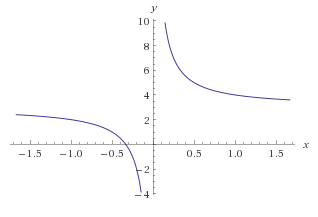
\includegraphics[scale=0.7]{figures/1_over_x_3.png}
        \vspace{2cm}
\end{enumerate}


\bt{True or False. No justification necessary.}
\begin{enumerate}[resume]
    \item \underline{\hspace{1.52cm}} The horizontal asymptote of $\frac{4}{x-5} + 8$ is 8.
    \item \underline{\hspace{1.52cm}} If $\lim_{x \rightarrow c} f(x) = L$, then $L = f(c)$.
    \item \underline{\hspace{1.52cm}} If $L = h(a)$, then $\lim_{x \rightarrow a} h(x) = L$
    \item \underline{\hspace{1.52cm}} $g(x) = 2x$ exhibits exponential growth, because $g(x) \rightarrow \infty$ as $x \rightarrow \infty$ 
\end{enumerate}


\newpage

\section*{Solutions}
Write your answers in the space provided. No calculators allowed.

\bt{Explain and justify your thought process.}


    \begin{enumerate}
        \item Find $\lim_{x \rightarrow -5} \frac{\pi x^2-25\pi}{x+5}$\\
        \green{
        This is equivalent to 
        \eq{
        \lim_{x \rightarrow -5} \frac{\pi(x+5)(x-5)}{x+5} 
        & =  \lim_{x \rightarrow -5} \pi(x-5) = \pi (-5 -5) = -10 \pi, 
        }
        because the limit is concerned with $x$ close to, but not equal to $-5$.
        }
        \item Evaluate $\log_2(\log_3(\log_4 64))$ \\
        \green{
        These are nested functions. We feed $\log_4 64$ as an input into the next function $\log_3$. So we have
        $\log_4 64 = 3$\\
        $\log_3 3 = 1$ \\
        and finally $\log_2 1 = 0$.
        Therefore, the expression is equal to 0.
        }
        \item Explain the meaning of $\lim_{x \rightarrow a} f(x) = L$. \\
        \green{
        This means as $x$ approaches, but does not equal $a$, $f(x)$ gets close to L.
        }
    \end{enumerate}


\bt{No justification necessary.}

\begin{enumerate}[resume]
        \item For $f(x) = x^2 + 2$ and $g(x) = x + 5$, find all solutions to $3x = g(f(x))$.\\
    \green{
    Interpreting the notation, we have 
    \eq{
    3x = g(x^2 +2) = x^2 + 7.
    }
    So, $x^2 - 3x + 7 = 0$. This a quadratic, so we can complete the square: 
    $(x-1.5)^2 + 4.75 = 0$
    Since our function is $x^2$ shifted up by 4.75, it can never equal 0. 
    Therefore, there are no real solutions.
    }
    \item What are the minimum and maximum values of $x^2 + 10x + 77$?\\
    \green{
    To find the min and max, we related the function to $x^2$ by completing the square: 
    $$x^2 + 10x + 77 = (x+5)^2 + 52$$. 
    Therefore, the minimum is 52 and the maximum is $\infty$.
    }
    \item Does the graph below depict $a(x) = 1/x^3, b(x) = 3^{-x},$ $c(x) = 3^{x^2},$ or $d(x) = 1/x + 3$?
    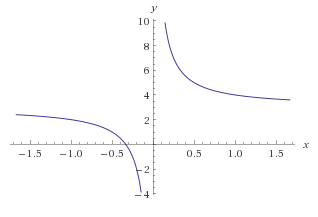
\includegraphics[scale=0.7]{figures/1_over_x_3.png}

    \green{
    The graph is the foundational function $1/x$ shifted up 3. Therefore, 
    it's the graph of $d(x)$.
    }
\end{enumerate}


\bt{True or False. No justification necessary.}
\begin{enumerate}[resume]
    \item \green{True} The horizontal asymptote of $\frac{4}{x-5} + 8$ is 8.
    \item \green{False} If $\lim_{x \rightarrow c} f(x) = L$, then $L = f(c)$.
    \item \green{False} If $L = h(a)$, then $\lim_{x \rightarrow a} h(x) = L$
    \item \green{False} $g(x) = 2x$ exhibits exponential growth, because $g(x) \rightarrow \infty$ as $x \rightarrow \infty$ 
\end{enumerate}
\end{document}

